\documentclass{article}
\usepackage[letterpaper, total={6.5in, 9in}]{geometry}
\usepackage[utf8]{inputenc}
\usepackage{verbatim}
\usepackage{graphicx}

\usepackage{biblatex} %Imports biblatex package
\addbibresource{references.bib} %Import the bibliography file

\title{Final Project: Network Protocol Check-a-roo}
\author{Jack Wilburn}
\date{April 2022}

\begin{document}

\maketitle

\section{Needham–Schroeder Protocol}

\begin{figure}[htbp]
  \centering
  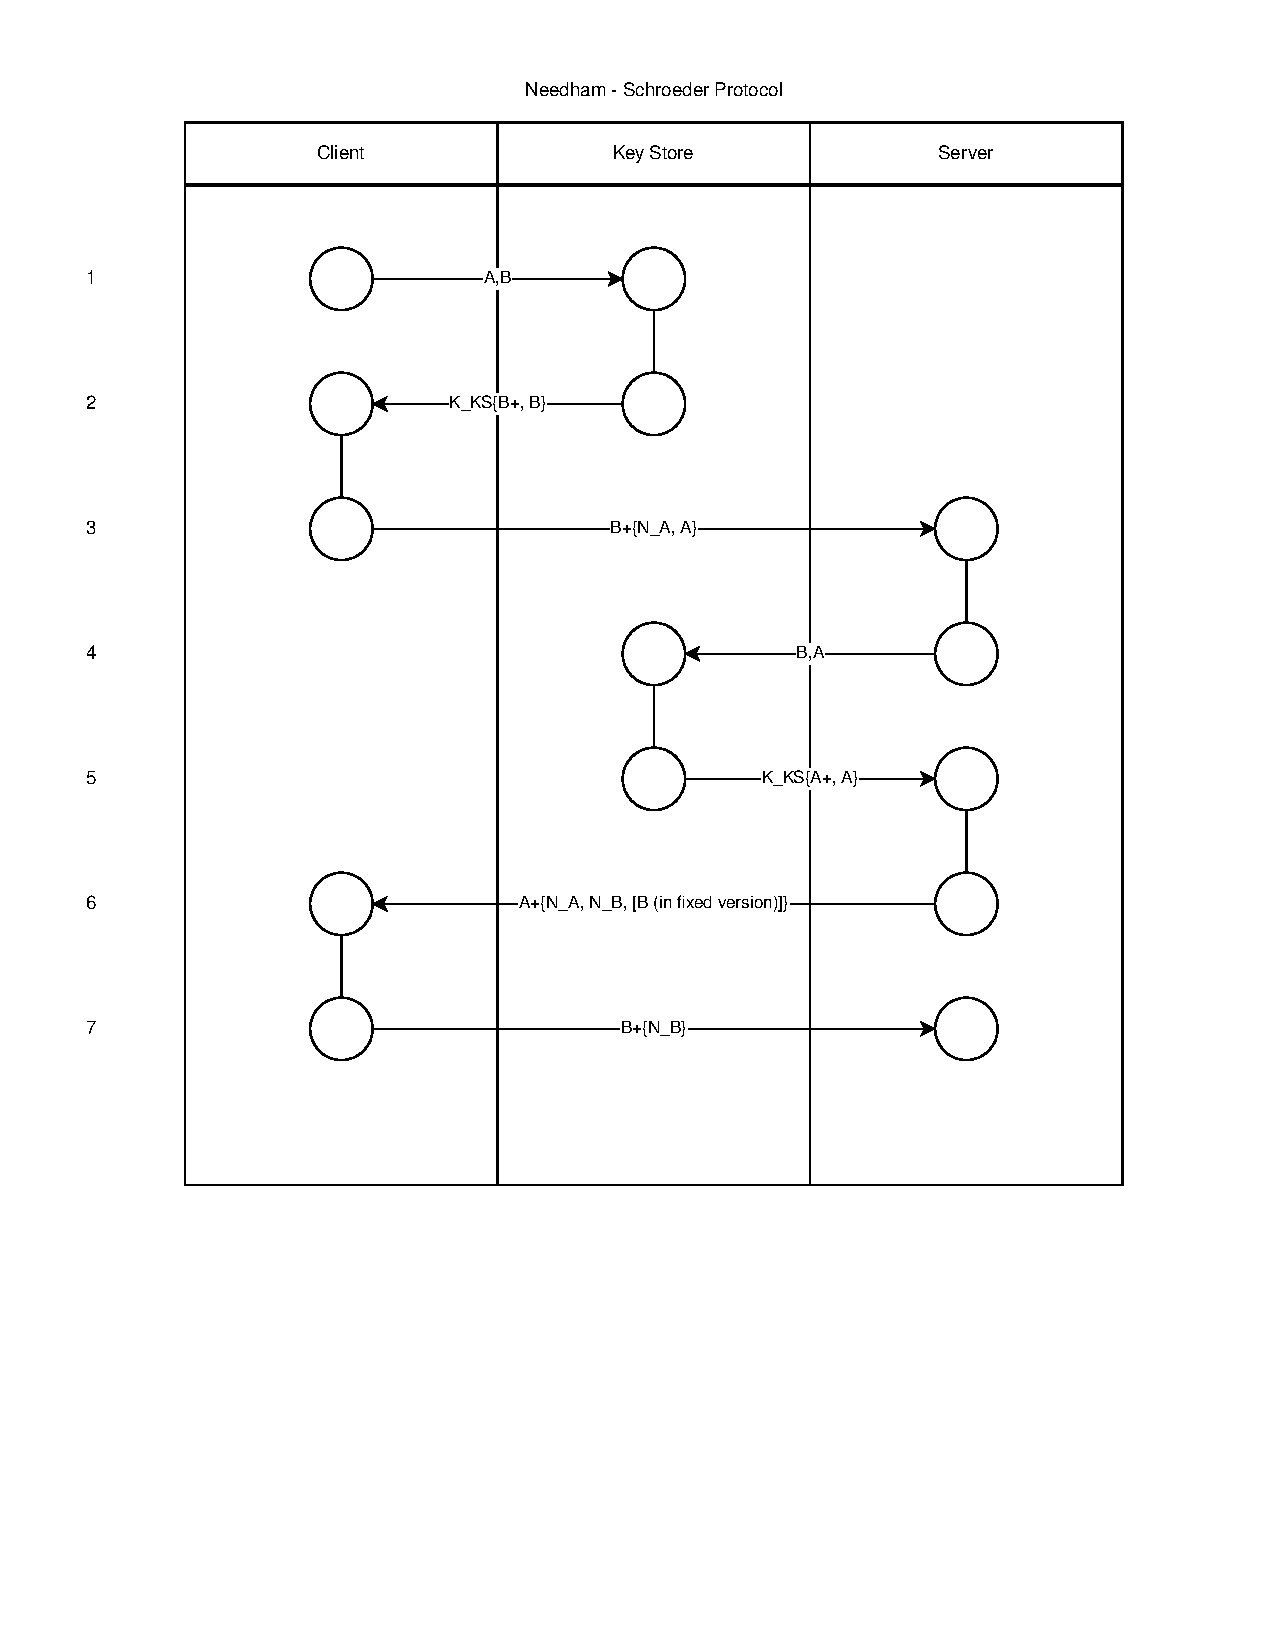
\includegraphics[width=300pt, height=400pt]{NS.pdf}
\end{figure}

The Needham-Schroeder protocol was designed by Roger Needham and Michael Schroeder for transporting keys intended for use over an insecure network. To review the software correctness of this protocol, I'm using the murphi model that was created by the Stanford Computer Security Laboratory \cite{stern}. This model only looks at three messages in the public-key version of the protocol, messages 3, 6, and 7. We only need to consider three messages in the protocol because those are the only ones that travel between the client and the server. The other messages are to the key store.

The model assumes that two legitimate parties communicate and one intruder attempts to find the transmitted secrets. The notes in the model claim that the "intruder always intercepts, [and that] agents only react to [an] intruder." There's also a fix that can be toggled to model an exploitable vulnerability, leading to different outputs at the end of model checking.

\subsection{The Modeled Messages}

\subsubsection{Message 3}

"A sends a nonce RA, together with A's name to B, encrypted with B's public key. B decrypts to get A's name and nonce."\cite{ns_protocol}

\subsubsection{Message 6}

"B generates a nonce RB and sends it together with RA to A, encrypted with KA. A decrypts the message. If it finds RA, it assumes that this is a message from B in response to its original message."\cite{ns_protocol}

\subsubsection{Message 7}

"A encrypts RB with KB and sends it to B. B decrypts the message. If it finds RB, it assumes that this is a message from A in response to its original message."\cite{ns_protocol}

\subsection{The Vulnerability and The Fix}

In 1995, Gavin Lowe authored a paper \cite{LOWE} that described a man-in-the-middle attack on the protocol, which arose from a weakness in message 6 in the protocol. This vulnerability violates the invariants, and the intruder tricks one of the legitimate parties (the client in the relationship). Like most man-in-the-middle attacks, the intruder tricks the client into thinking they're communicating with the server while there is an intermediary intercepting the messages.

The fix for the vulnerability is to include an additional piece of information in the message, the server's identity. This extra piece of data is then encrypted with the client's public key so only they can decrypt the message. This ensures that you will see the server identifier and kill the connection to the intermediary if not you're communicating with the server. Applying this fix in the murphi code leads to the invariants remaining un-violated.


\subsection{Rumur/Murphi Commands I Used}

The Murphi code I downloaded from the Stanford Computer Security Laboratory was not compatible with rumur-2021-12-27. Rumur was complaining about types on a lot of lines, and I decided to pivot to using cmurphi 5.5.0. I downloaded it from the website and set it up and ran the following commands:

\begin{verbatim}
cmurphi5.5.0/src/mu needham-schroeder.m 
g++ needham-schroeder.cpp -I cmurphi5.5.0/include/
./a.out -ndl
# ndl means don't check deadlock. It seems the implementation has a
# loop that triggers the deadlock 

# Without fix:
Result:
    Invariant "initiator correctly authenticated" failed.
State Space Explored:
    964 states, 2306 rules fired in 0.10s.


# With fix:
Status:
    No error found.
State Space Explored:
    980 states, 2314 rules fired in 0.10s.
\end{verbatim}











\clearpage

\section{OpenID 2.0}

\begin{figure}[htbp]
  \centering
  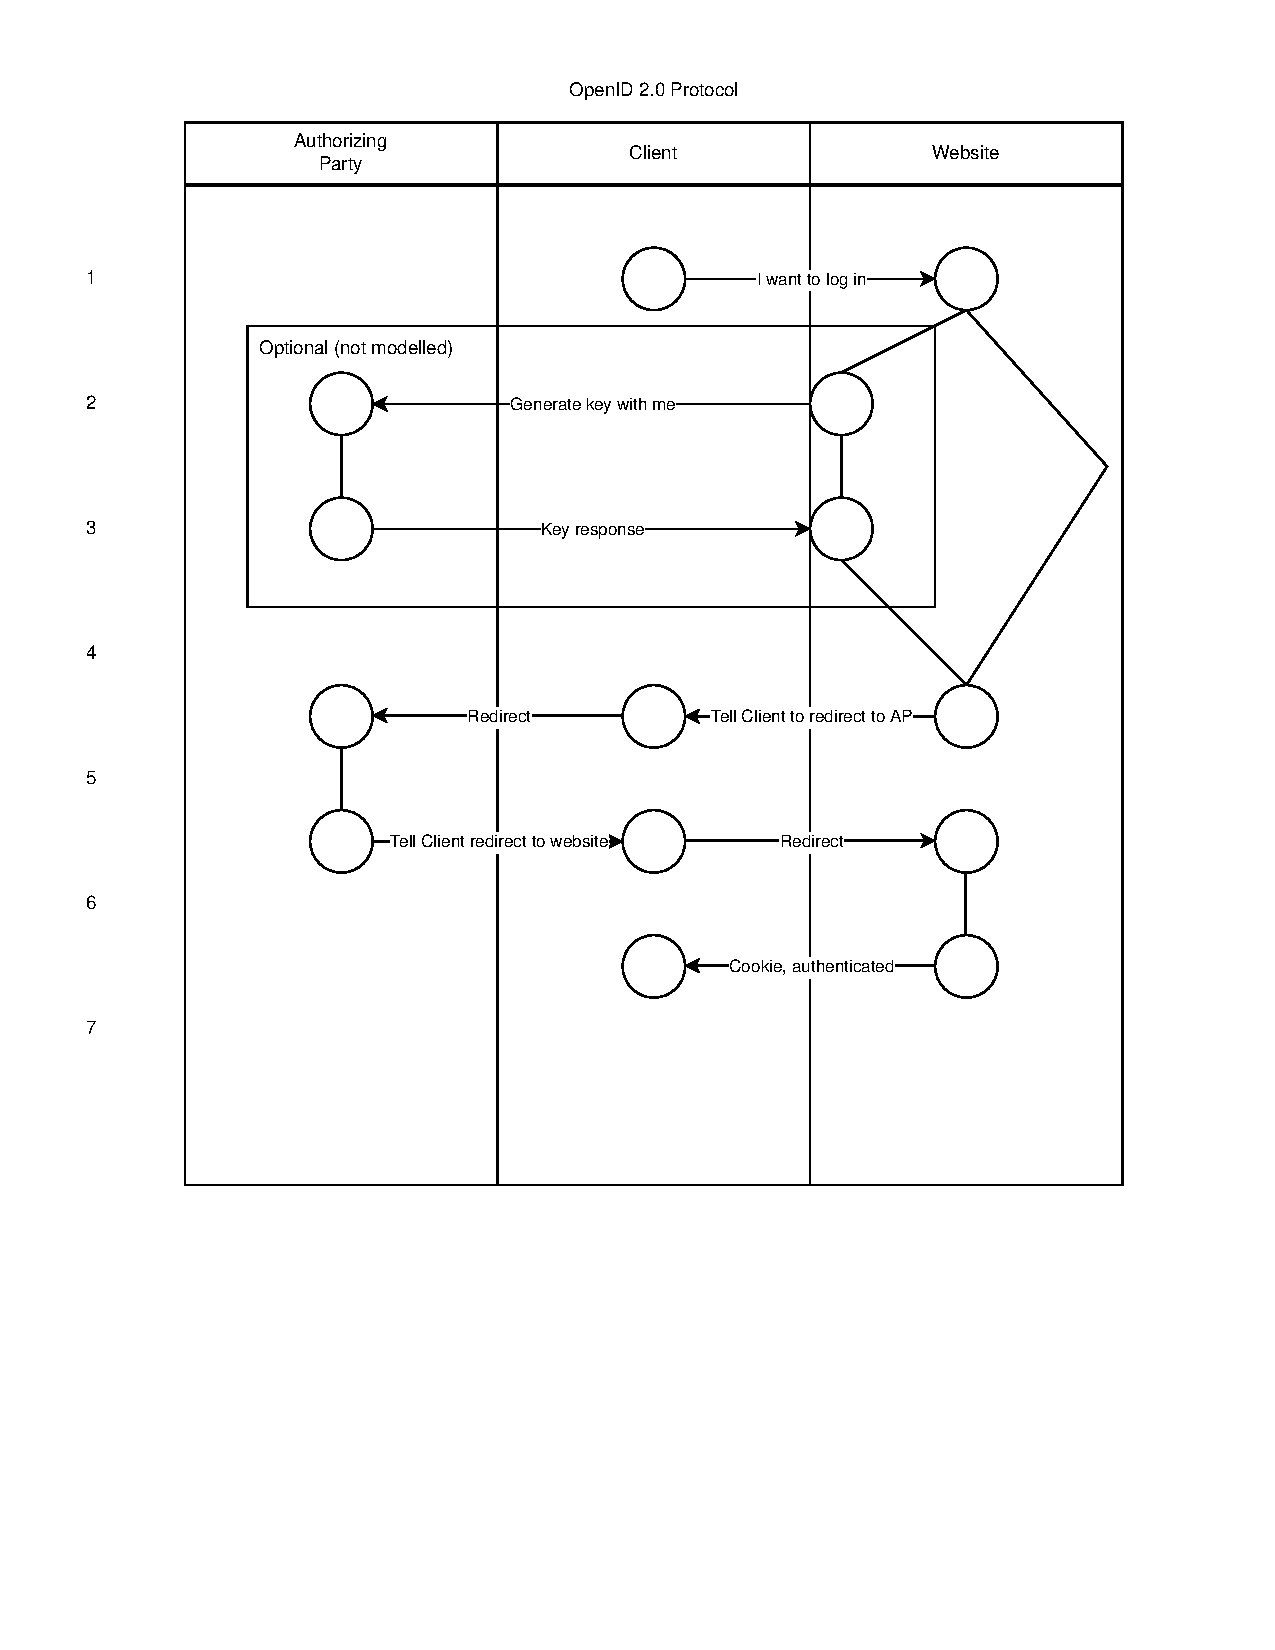
\includegraphics[width=300pt, height=400pt]{OpenID.pdf}
\end{figure}

The OpenID 2.0 protocol "provides a way to prove that an end-user controls an Identifier" \cite{lingamneni_newman}. This means that the protocol can verify that users are whom they say they are by proving they are allowed to access an identifier held by a third party. Ultimately, using this protocol means a user can authenticate with a service without ever having to enter a user id or password on that server; instead, a third party provides the authentication.

We use this technology frequently, for example, with the sign in with your Google/GitHub/ORCID/etc. account button. Since this protocol is so heavily relied upon, it must be verifiably correct. To this end, the Stanford Computer Security Laboratory created a murphi model that checks the correctness of the protocol to ensure that we genuinely are protected by the protocol we depend on.

\subsection{The Modelled Messages}

This model considers most messages in the OpenID 2.0 protocol, except the option message between the website a user would be trying to authenticate with and the authentication/OAuth provider. The supporting documentation for the model claims that this is unnecessary since it should already rely on checked protocols to provide a secure communication channel (Diffie-Hellman, etc.).

The messages that the model covers are the authentication requests to the website and the authentication provider, the responses from the provider, and the redirects that the user would experience during the authentication flow. See the diagram above for the modeled messages.

\subsection{The Vulnerability and The Fix}

The proposed vulnerability that this murphi code models is a cross-site request forgery sent by an intruder who can control a client's browser. The attack generates all the messages in the protocol but waits to send the last one to the website the user is trying to authenticate with until the legitimate user is trying to log in. Since the intruder sends their message instead of the legitimate user, the user authenticates as the intruder. While this attack vector is unlikely ever to be exploited in the wild, unless an intruder wants a legitimate user to access the intruder's info/files, it shows that the protocol is not perfectly sound. It's possible to break the protocol by injecting messages at the right point, which it really shouldn't be.

\subsection{Rumur/Murphi Commands I Used}

The Murphi code I downloaded from the Stanford Computer Security Laboratory was not compatible with rumur-2021-12-27. Rumur was complaining about types on a lot of lines, so, again, I used cmurphi 5.5.0. I then ran the following commands:

\begin{verbatim}
cmurphi5.5.0/src/mu openid2.m 
g++ openid2.cpp -I cmurphi5.5.0/include/
./a.out -ndl -m 2048
# -ndl means don't check deadlock. It seems the implementation has a
# loop that triggers the deadlock again.
# -m increases the memory limit for the closed hash table


# How code from SecLab ran:
Result:
    Invariant "initiator correctly authenticated" failed.
State Space Explored:
    865 states, 1311 rules fired in 1.01s.
\end{verbatim}

I had to toggle a flag in the code to turn the vulnerability off, that is disable an intruder from sending that message in place of the legitimate user. In this configuration, I got the following output showing that there were no other violations found in the model of the protocol:

\begin{verbatim}
# After the fix, the output was:
Status:
    No error found.
State Space Explored:
    854076 states, 1904227 rules fired in 54.68s.
\end{verbatim}











\clearpage

\section{CCN}

For my other class, CS 6490 Network Security, I'm implementing a model proposed by researchers at PARC \cite{ccn} called CCN (Content Centric Networking). It is a paradigm shift in how we consider computer connectivity, a complete departure from IP routing. Instead of a client requesting to go to a specific machine that it knows by IP address (or URL that is DNS resolved to an IP address), clients request data, and intermediary routers figure out the fastest way to fetch the information. You no longer have to use an IP address; instead, routers figure out who has the data and ask them for it. Each response is cached on every node so that anyone else requesting the same data will receive a faster, cached response. Also, nodes aggregate requests, so DDOS attacks are much less likely because of the reduced amount of traffic on the network. There are other perks, such as when deploying websites since the entire network is a CDN, which would yield faster performance than one static server as we often have with IP routing.

I haven't seen any formal model checking with the early-stage code and proof of concept libraries. I thought it would be fun to code it up in one of our model checking tools and ensure there were no flaws in my understanding of the protocol and the protocol itself. I chose Alloy since I'm most familiar with it, and I prefer the interface.

\subsection{The Things I Chose To Model}

There are a couple of fantastic pieces of the CCN node architecture, including the cache and PIT (pending interest table), that I wanted to model. These pieces of the protocol/implementation lead to reduced traffic on the network. The cache keeps content closer to clients so they don't have to travel across the network, and nodes use the PIT to remember who is waiting for the same content so the node can send just one packet upstream. This can bring substantially better performance and significantly reduce network traffic, especially when lots of clients want the same information.

In choosing to model these two pieces of the Node architecture, I had to model some additional components, such as the data itself, client requests, etc. The full details are in the file CCN.als. I wrote several checks to run on a small network to verify that all nodes can reach all data on the network and that pending interests are configured correctly.

\subsection{Alloy Commands I Used}

After loading up the model, you should be able to run the model checking code and generate some acceptable models. I modeled several nodes and their communications to make the state space interesting. It was essential to make a decent-sized topology to see how the network would behave in real-world circumstances. The predicates are combined and ran, and I manually checked each of the predicates as an assert statement for the same size networks. 

\centering
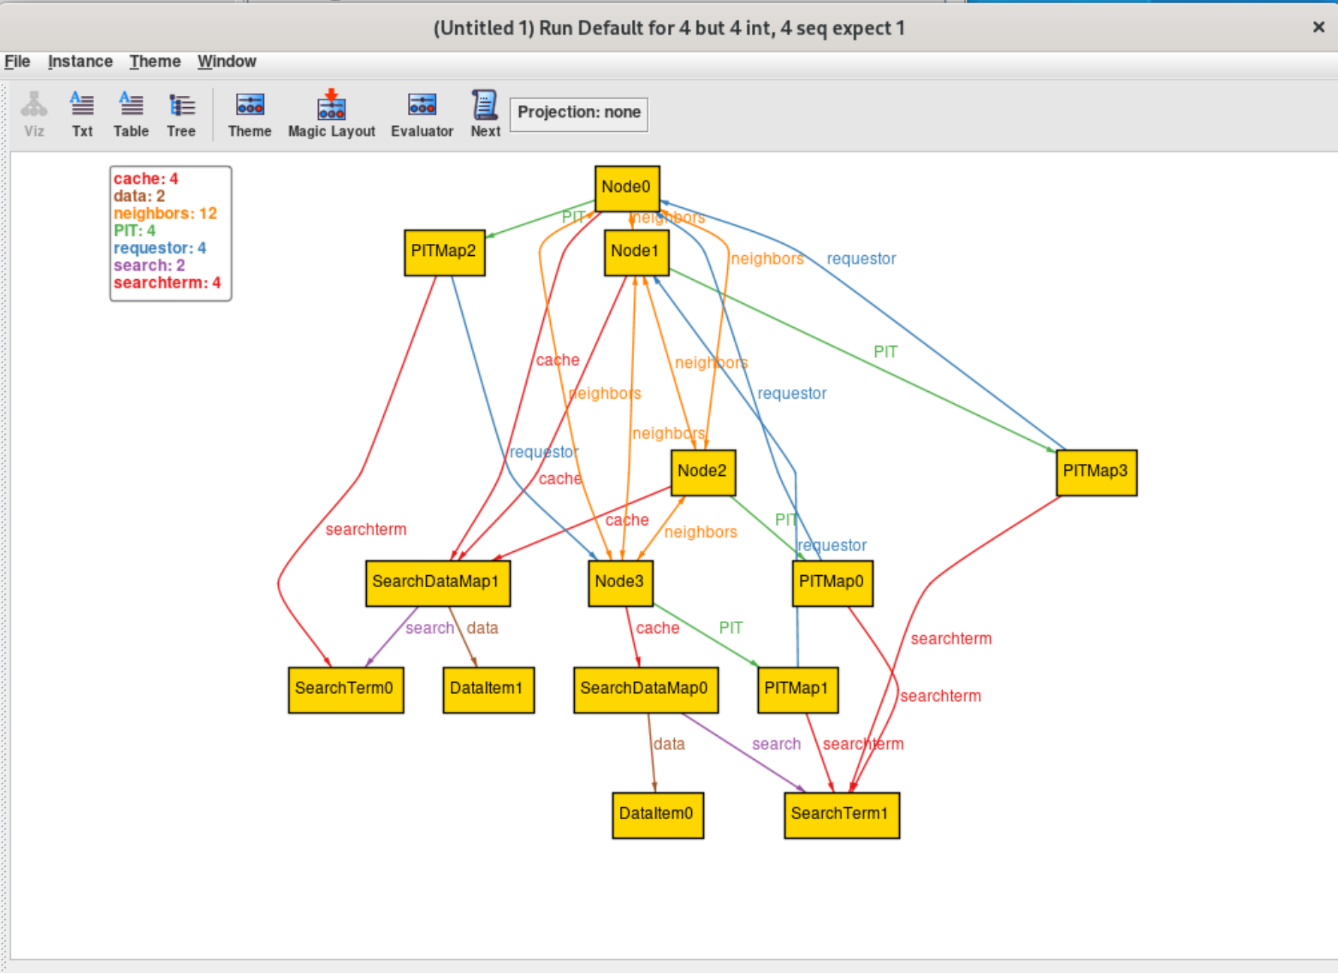
\includegraphics[scale=0.25]{CCN.png}

\clearpage
\printbibliography

\end{document}
